\section{实验七:Network driver}\label{sec:Network_driver}

为网络接口卡 (NIC) 编写一个 xv6 设备驱动程序。

\subsection{实验目的}

\begin{enumerate}
	\item 理解内核网络栈与硬件的接口边界:熟悉以太网/ARP/IP/UDP 报文封装关系,掌握 E1000 的 MMIO 寄存器、Tx/Rx 描述符环(TDT/TDH、RDT/RDH)与 DMA 工作机制。
	\item 能够在 xv6 中实现并验证网卡收发路径:完成 \texttt{e1000\_transmit()} 与 \texttt{e1000\_recv()},正确使用锁与内存屏障,处理中断并推动环形队列前移,使数据包能从应用层下发至 NIC、从 NIC 回送至 \texttt{net\_rx}。
	\item 掌握驱动调试与验证方法:在 QEMU 环境下通过提供的测试用例与日志/寄存器打印定位问题,观测丢包与竞态并进行修正,形成可复现的验证流程。
\end{enumerate}

\subsection{实验内容}

完成 \texttt{e1000\_transmit()} 和 \texttt{e1000\_recv()} ,两者均在 kernel/e1000.c 中,以便驱动程序可以发送和接收数据包。

\subsection{实验准备}

阅读 xv6 参考书的第 5 章,阅读 E1000 软件开发手册的第 2、3、13、14 章

\subsubsection{网络结构与协议}

\begin{enumerate}
	\item 以太网(Ethernet):局域网(Local Area Network)下各个主机都是通过以太网进行连接。以太网帧结构:start flag + 48位目标eth地址 + 48位源eth地址 + 16位ether type(payload中的数据协议类型)+ payload + end flag,如\cref{lst:eth} 所示。互联网下各个LAN 通过路由器之间的 TCP/IP 协议连接。
	\item ARP:以太网协议足以将 packet 在 LAN 中传送,但是如果需要将 packet 传送给远程 Host,需要 IP 地址。ARP 协议是将 IP 地址翻译为 eth 地址的协议,嵌套在 ethernet packet 中 ( 即 ether header 后面就是 ARP header,ARP header 是 ether header 的 payload ),ARP header 请求一个 IP 地址对应的 eth 地址,这个 ARP header 会被所有 LAN 内的 host 接收,对应的 Host 将返回 IP 地址。
	\item IP:IP 数据包的 ethernet type=0x0800,IP header 中包括了 32 位的 IP 地址,高位的 IP 地址是 network number 来帮助 router 将 packet 进行转发,protocol number 让接收者知道这个 IP packet 的更高级协议是什么。在 packet 从一个 router 转发到另一个 router 的过程中,ether header 会被除去,但是 IP header 一直是保留着的。
	\item UDP:UDP 是传输层协议,根据 sockets API 规定了当一个 packet 到达正确 host 时需要被发送到的端口号,操作系统将把这个端口号上获取的 packets 作为一个 file descriptor 以供进程读取。端口号 53 是 DNS server 指定的端口号。
\end{enumerate}

\begin{figure}[!htb]
	\centering
	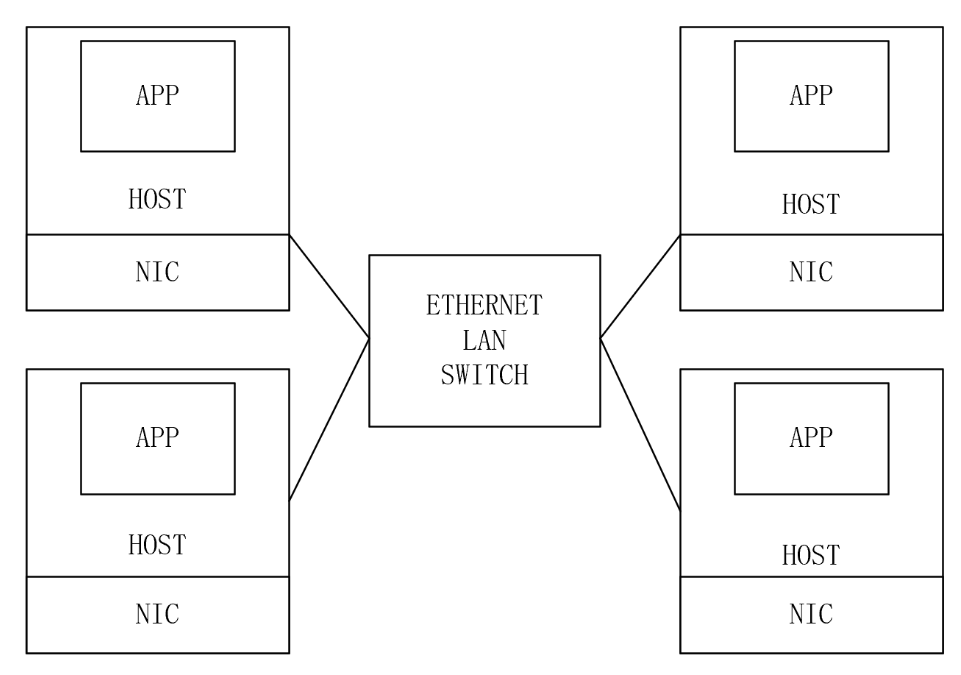
\includegraphics[width=0.6\textwidth]{Ethernet}
	\caption{基于以太网交换机的局域网拓扑}
	\label{fig:Ethernet}
\end{figure}

\begin{figure}[!htb]
	\centering
	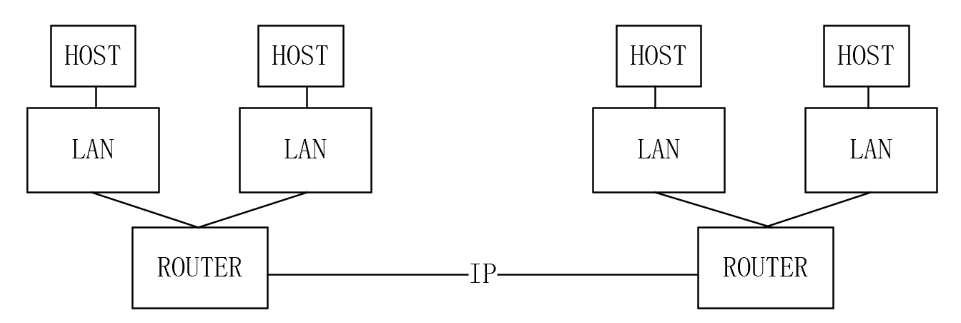
\includegraphics[width=0.6\textwidth]{router}
	\caption{路由器互联的多局域网 IP 网络拓扑}
	\label{fig:router}
\end{figure}

\begin{listing}[!htb]
	\begin{minted}{c}
// an Ethernet packet header (start of the packet).
struct eth {
    uint8  dhost[ETHADDR_LEN];
    uint8  shost[ETHADDR_LEN];
    uint16 type;
} __attribute__((packed));
	\end{minted}
	\caption{eth 结构体}\label{lst:eth}
\end{listing}

\begin{listing}[!htb]
	\begin{minted}{c}
// an ARP packet (comes after an Ethernet header).
struct arp {
    uint16 hrd; // format of hardware address
    uint16 pro; // format of protocol address
    uint8  hln; // length of hardware address
    uint8  pln; // length of protocol address
    uint16 op;  // operation
    
    char   sha[ETHADDR_LEN]; // sender hardware address
    uint32 sip;              // sender IP address
    char   tha[ETHADDR_LEN]; // target hardware address
    uint32 tip;              // target IP address
} __attribute__((packed));

#define ARP_HRD_ETHER 1 // Ethernet

enum {
    ARP_OP_REQUEST = 1, // requests hw addr given protocol addr
    ARP_OP_REPLY = 2,   // replies a hw addr given protocol addr
};
	\end{minted}
	\caption{arp 结构体}\label{lst:arp}
\end{listing}

\begin{listing}[!htb]
	\begin{minted}{c}
// an IP packet header (comes after an Ethernet header).
struct ip {
    uint8  ip_vhl; // version << 4 | header length >> 2
    uint8  ip_tos; // type of service
    uint16 ip_len; // total length
    uint16 ip_id;  // identification
    uint16 ip_off; // fragment offset field
    uint8  ip_ttl; // time to live
    uint8  ip_p;   // protocol
    uint16 ip_sum; // checksum
    uint32 ip_src, ip_dst;
};
	\end{minted}
	\caption{ip 结构体}\label{lst:ip}
\end{listing}

\begin{listing}[!htb]
	\begin{minted}{c}
// a UDP packet header (comes after an IP header).
struct udp {
    uint16 sport; // source port
    uint16 dport; // destination port
    uint16 ulen;  // length, including udp header, not including IP header
    uint16 sum;   // checksum
};
	\end{minted}
	\caption{UDP 结构体}\label{lst:UDP}
\end{listing}

\subsubsection{内核网络堆栈}

内核网络堆栈的结构如\cref{fig:kernel_network_stack} 所示。

最底层是 NIC 硬件,由 NIC 驱动负责中断、DMA 与收发队列管理;其上是网络层 IP,负责路由、分片/重组与把报文分发给传输层,并配合 ARP 在同一链路上完成 IP→MAC 的解析;传输层包含 UDP(无连接、尽力而为)与 TCP(面向连接、可靠传输、拥塞/流量控制),二者按端口或连接四元组将数据与 socket 关联;最上层是应用(如浏览器、DNS)通过 socket 系统调用与内核通信。数据发送路径为 App→socket→UDP/TCP→IP(+ARP)→驱动→NIC,接收路径相反。

\begin{figure}[!htb]
	\centering
	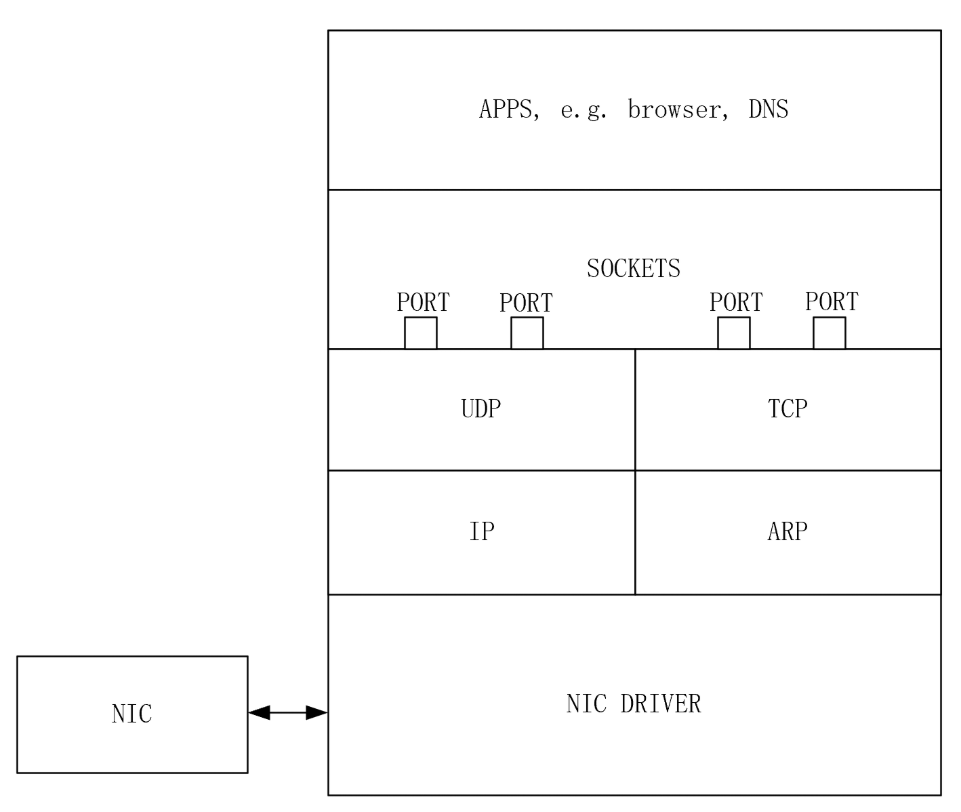
\includegraphics[width=0.55\textwidth]{kernel_network_stack}
	\caption{内核网络堆栈结构图}
	\label{fig:kernel_network_stack}
\end{figure}

\subsubsection{硬件结构概述}

E1000 网卡基本结构如\cref{fig:E1000} 所示,包括 OSI 模型的2个层:物理层和数据链路层。物理层由 PHY 芯片控制,定义了数据传送与接收所需要的光电信号、时钟基准等。数据链路层由 MAC 芯片控制,提供寻址机构、数据帧的构建、向网络层提供标准数据接口等功能。

\begin{figure}[!htb]
	\centering
	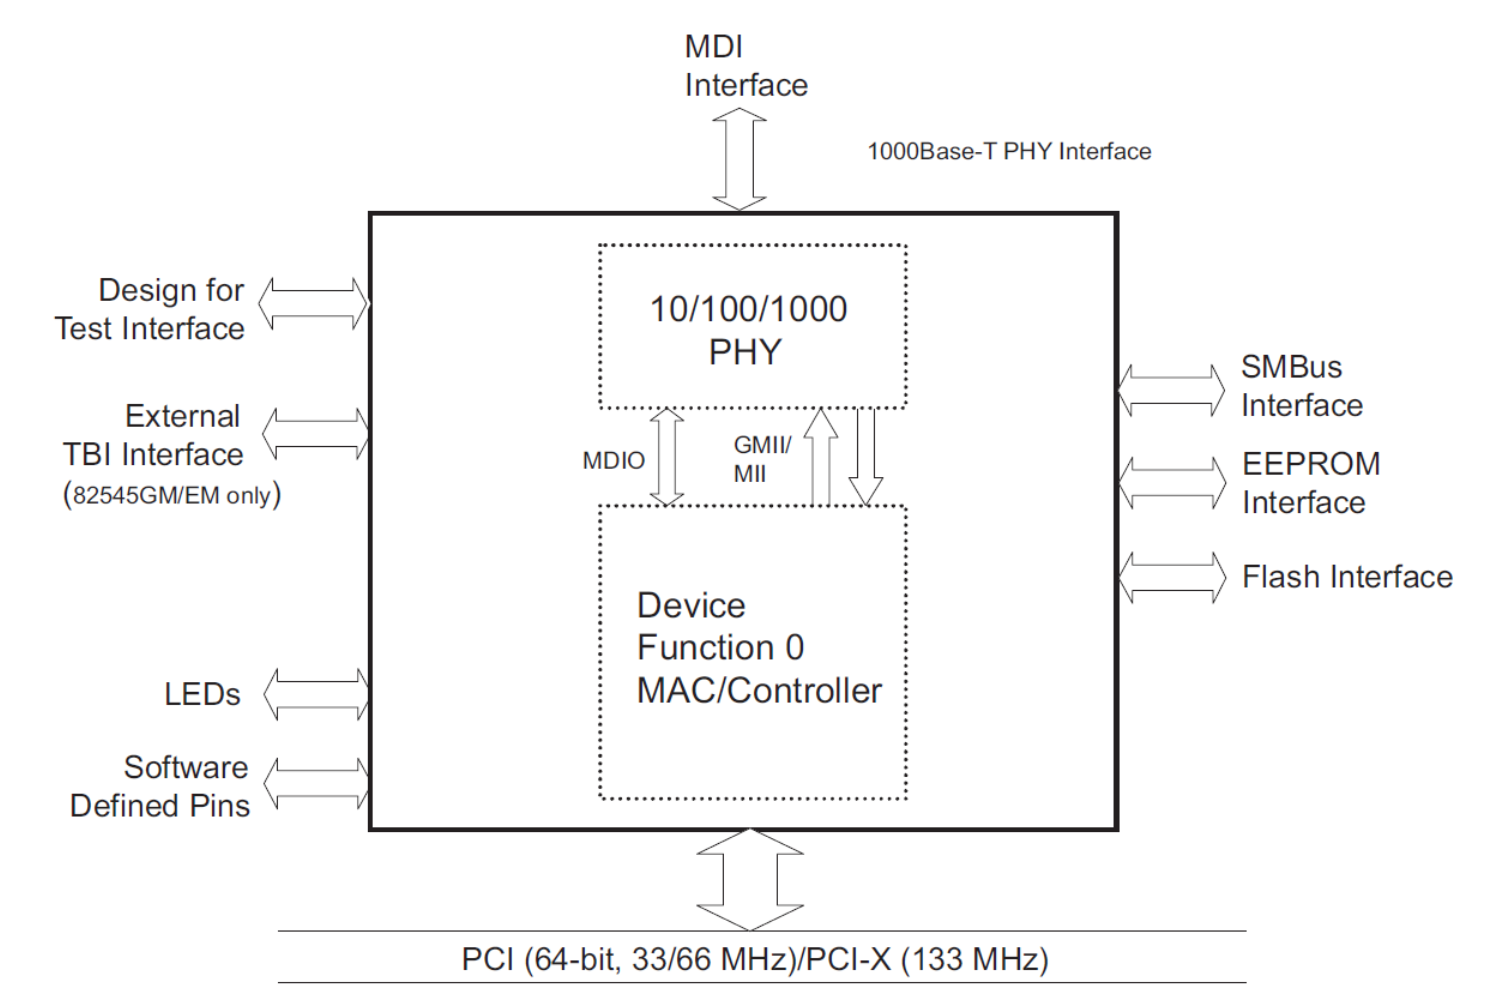
\includegraphics[width=0.65\textwidth]{E1000}
	\caption{E1000 网卡基本结构}
	\label{fig:E1000}
\end{figure}

DMA(Direct Memory Access) 是可以不通过 CPU 直接访问内存的机制,在进行 DMA 传输时 DMA Engine 控制 PCI 总线,将内存中的数据和 FIFO data buffer (64KB)中的数据互传。

\begin{figure}[!htb]
	\centering
	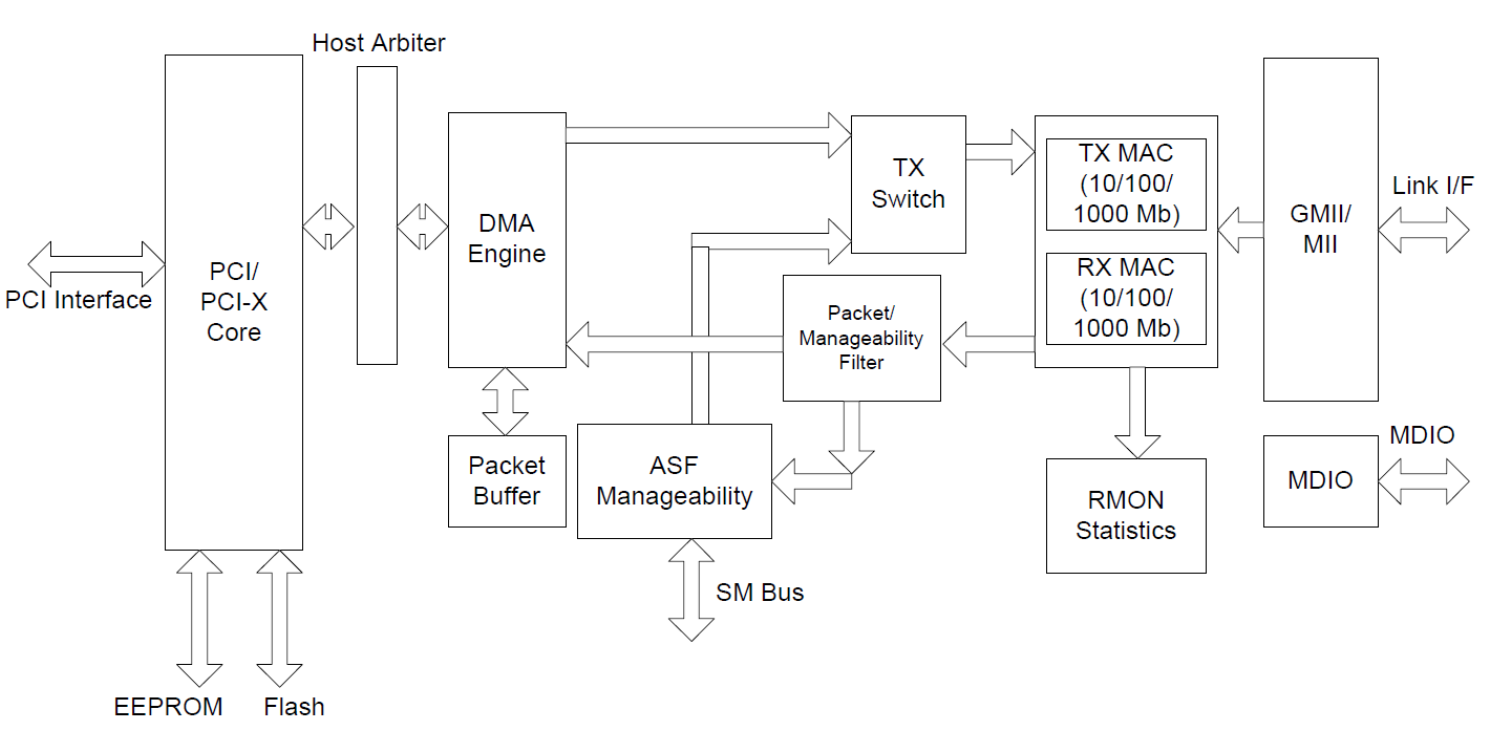
\includegraphics[width=0.65\textwidth]{PCI_MAX}
	\caption{PCI/PCI-X 核心接口}
	\label{fig:PCI_MAX}
\end{figure}

\subsubsection{接收和发送}

数据发送时,CPU 将 IP 数据包打包放入内存中,通知 DMA Engine 进行 DMA 传输,数据放入 FIFO data buffer 中。MAC 将 IP 数据包拆分为最小 64KB,最大 1518KB 的数据帧,每一帧包含了目标 MAC 地址、自己的 MAC 地址和数据包中的协议类型以及 CRC 校验码。目标 MAC 地址通过 ARP 协议获取。PHY 接受 MAC 传送的数据,将并行数据转化为串行数据后进行编码,在转变为模拟信号将数据进行传输。

RAM 中的 tx/rx buffer(接收/发送缓冲区)是一个环形结构,有 head 和 tail 两个指针,其中 head 的位置由网卡控制。在进行发送时,每发送完成一个 packet 数据包,网卡就会自动将 head 向前移动一个 mbuf,而需要将某个 packet 发送时,软件将 tail 向前移动一个 mbuf;在进行接收时,每接收到一个 packet 网卡自动将 head 向前移动一个 mbuf,软件读取 tail 所指向的 mbuf,并向前移动。移动到最后一个 mbuf 后从头开始,形成一个环形缓冲区的结构。

\begin{figure}[!htb]
	\centering
	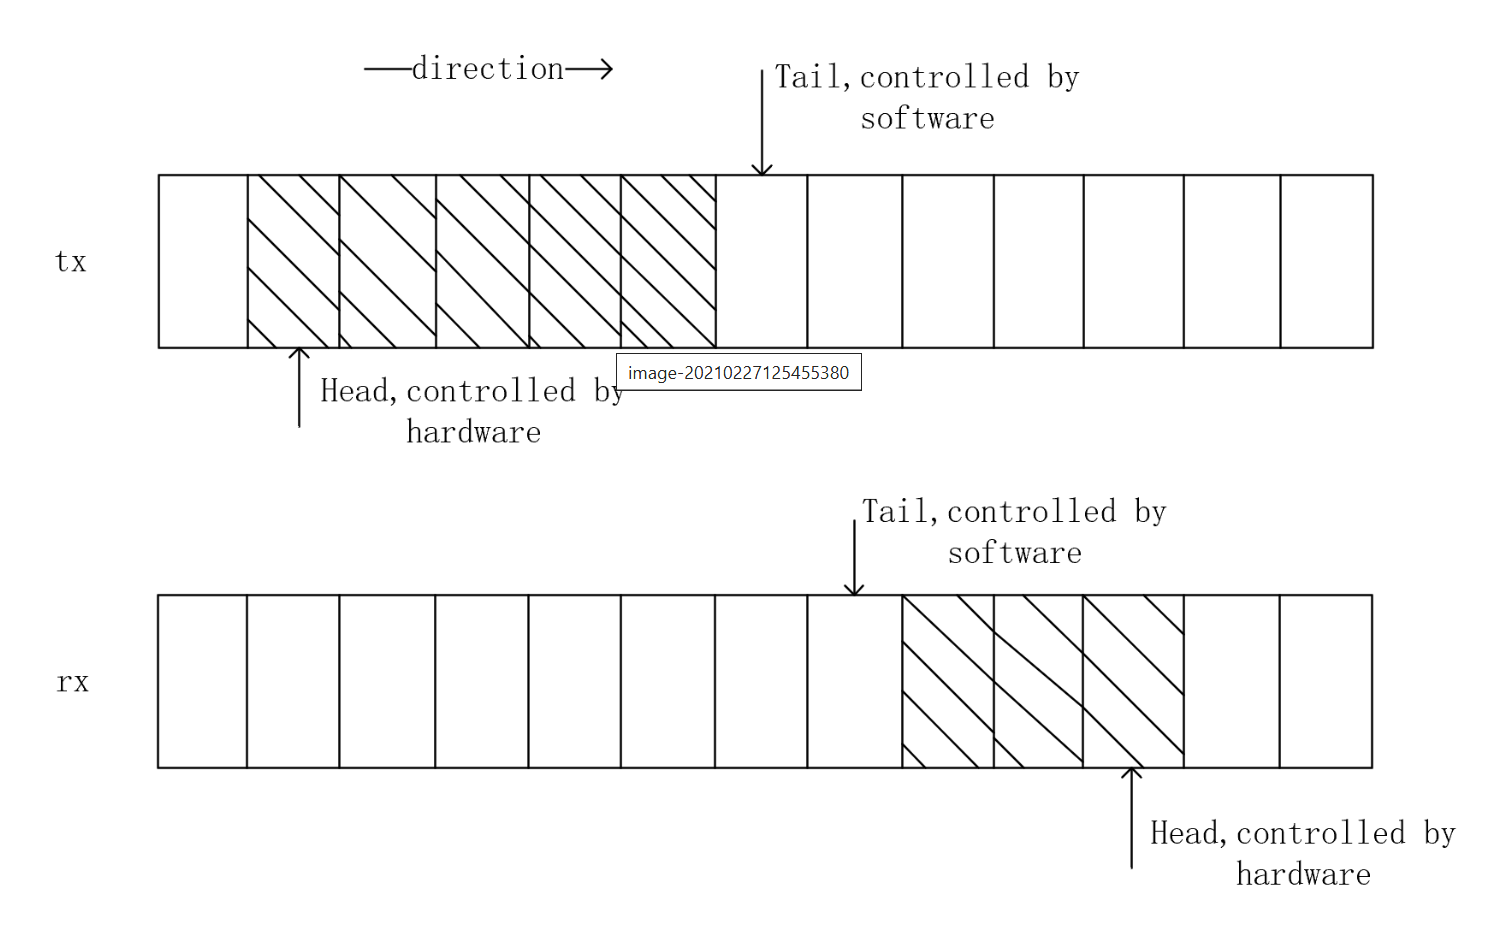
\includegraphics[width=0.65\textwidth]{Ring}
	\caption{tx/rx buffer 的变化}
	\label{fig:Ring}
\end{figure}

\begin{figure}[!htb]
	\centering
	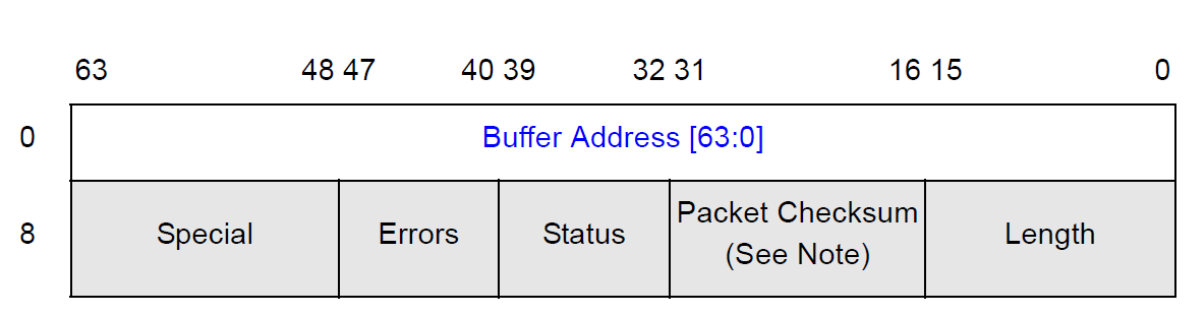
\includegraphics[width=0.65\textwidth]{receive_descriptor_layout}
	\caption{接收描述符的格式}
	\label{fig:receive_descriptor_layout}
\end{figure}

descriptor结构是在网卡的寄存器中的,用于描述每一个RAM中的mbuf

\subsection{实验过程}

\subsubsection{实现 e1000\_transmit}

\begin{enumerate}
	\item 读取 \texttt{ E1000\_TDT } 得到环索引 \texttt{ next\_tx\_idx }。
	\item 若 \texttt{ tx\_ring[next\_tx\_idx].status } 无 \texttt{ E1000\_TXD\_STAT\_DD },返回 \texttt{ -1 }。
	\item 若旧 \texttt{ mbuf } 存在,\texttt{ mbuffree(tx\_mbufs[next\_tx\_idx]) }。
	\item 填写 \texttt{ addr = m->head }、\texttt{ length = m->len }、\texttt{ cmd = EOP|RS },并保存 \texttt{ m } 到 \texttt{ tx\_mbufs }。
	\item \texttt{ \_sync\_synchronize() } 后,更新 \texttt{ E1000\_TDT = (next\_tx\_idx + 1) \% TX\_RING\_SIZE }。
	\item 成功返回 \texttt{ 0 },无可用描述符则 \texttt{ -1 }。
\end{enumerate}

\begin{listing}[!htb]
	\begin{minted}{c}
int
e1000_transmit(struct mbuf *m)
{
    acquire(&e1000_lock);
    // 获取下一个环索引
    int next_tx_idx = regs[E1000_TDT];
    // 检查索引到的位置E1000有没有完成先前的传输请求
    if((tx_ring[next_tx_idx].status & E1000_TXD_STAT_DD) == 0){
        release(&e1000_lock);
        return -1;
    }
    // 检查用于传输上一个包的缓冲区是否被释放
    else if(tx_mbufs[next_tx_idx] != 0){
        // 释放缓冲区
        mbuffree(tx_mbufs[next_tx_idx]);
    }

    // 填写描述符字段
    tx_ring[next_tx_idx].addr = (uint64) m->head;
    tx_ring[next_tx_idx].length = m->len;
    tx_ring[next_tx_idx].cmd = E1000_TXD_CMD_EOP | E1000_TXD_CMD_RS;
    tx_mbufs[next_tx_idx] = m;
    // 内存屏障,防止指令重排
    __sync_synchronize();
    regs[E1000_TDT] = (next_tx_idx + 1) % TX_RING_SIZE;
    if(&tx_ring[next_tx_idx].status == 0 || tx_mbufs[next_tx_idx] == 0){
        release(&e1000_lock);
        return -1;
    }
    release(&e1000_lock);
    return 0;
}
	\end{minted}
	\caption{实现 e1000\_transmit}\label{lst:e1000_transmit}
\end{listing}

\subsubsection{实现 e1000\_recv}

\begin{enumerate}
	\item 计算 \texttt{ next\_rx\_idx = (E1000\_RDT + 1) \% RX\_RING\_SIZE }。
	\item 若 \texttt{ rx\_ring[next\_rx\_idx].status } 无 \texttt{ E1000\_RXD\_STAT\_DD },停止。
	\item 设 \texttt{ rx\_mbufs[next\_rx\_idx]->len = rx\_ring[next\_rx\_idx].length },调用 \texttt{ net\_rx(...) }。
	\item 用 \texttt{ mbufalloc(0) } 补新 \texttt{ mbuf },更新 \texttt{ addr },清 \texttt{ status = 0 }。
	\item \texttt{ \_sync\_synchronize() } 后,写回 \texttt{ E1000\_RDT = next\_rx\_idx }。
\end{enumerate}

\begin{listing}[!htb]
	\begin{minted}{c}
static void
e1000_recv(void)
{
    while(1){
        uint32 next_rx_idx = (regs[E1000_RDT]+1) % RX_RING_SIZE;
        if((rx_ring[next_rx_idx].status & E1000_RXD_STAT_DD) == 0){
            break;
        }
        rx_mbufs[next_rx_idx]->len = rx_ring[next_rx_idx].length;
        net_rx(rx_mbufs[next_rx_idx]);
        rx_mbufs[next_rx_idx] = mbufalloc(0);
        
        // 如果申请失败,则panic
        if (!rx_mbufs[next_rx_idx])
            panic("e1000");
        rx_ring[next_rx_idx].addr = (uint64) rx_mbufs[next_rx_idx]->head;
        rx_ring[next_rx_idx].status = 0;
        // 内存屏障,防止指令重排
        __sync_synchronize();
        regs[E1000_RDT] = next_rx_idx;
    }
}
	\end{minted}
	\caption{实现 e1000\_recv}\label{lst:e1000_recv}
\end{listing}

\subsection{实验小结}

本实验在 e1000.c 中完成了基于环形队列的网卡驱动收发路径。初始化阶段通过 e1000\_init 建立 TX/RX 描述符环(大小 16),为 RX 环预分配 mbuf 并把 addr 指向 mbuf->head,配置关键寄存器(TDBAL/TDLEN/TDH/TDT、RDBAL/RDLEN/RDH/RDT、TCTL/TIPG、RCTL 等)。发送路径 e1000\_transmit 在加锁后读取 TDT 取得当前槽位,若未见 E1000\_TXD\_STAT\_DD 则说明硬件未回写、返回 -1;否则释放旧 mbuf,填入 addr/length/cmd(EOP|RS) 并保存 mbuf 指针,执行内存屏障保证可见性,再将 TDT 前移并取模,实现无缝循环复用。

接收路径 e1000\_recv 在中断 e1000\_intr 触发后被调用,先清 ICR 再使用循环从 (RDT+1)\%RX\_RING\_SIZE 开始检查 E1000\_RXD\_STAT\_DD,若有新包则把描述符长度写入 mbuf->len 并交给 net\_rx;随后用 mbufalloc(0) 补一个新 mbuf,更新描述符 addr、清零 status,执行内存屏障并写回 RDT,告知硬件该槽可复用。整个实现依赖环索引取模处理超过环大小的累计包量,利用 DD 位与内存屏障确保硬件/软件同步,结合中断驱动保证高效且正确的包收发。